% ------------------------------------------------------------
% Pandoc Default Begins

% Options for packages loaded elsewhere
\PassOptionsToPackage{unicode}{hyperref}
\PassOptionsToPackage{hyphens}{url}
%
\documentclass[
]{article}
\usepackage{lmodern}
\usepackage{amssymb,amsmath}
\usepackage{ifxetex,ifluatex}
\ifnum 0\ifxetex 1\fi\ifluatex 1\fi=0 % if pdftex
	\usepackage[T1]{fontenc}
	\usepackage[utf8]{inputenc}
	\usepackage{textcomp} % provide euro and other symbols
\else % if luatex or xetex
	\usepackage{unicode-math}
	\defaultfontfeatures{Scale=MatchLowercase}
	\defaultfontfeatures[\rmfamily]{Ligatures=TeX,Scale=1}
\fi
% Use upquote if available, for straight quotes in verbatim environments
\IfFileExists{upquote.sty}{\usepackage{upquote}}{}
\IfFileExists{microtype.sty}{% use microtype if available
	\usepackage[]{microtype}
	\UseMicrotypeSet[protrusion]{basicmath} % disable protrusion for tt fonts
}{}
\makeatletter
\@ifundefined{KOMAClassName}{% if non-KOMA class
	\IfFileExists{parskip.sty}{%
		\usepackage{parskip}
	}{% else
		\setlength{\parindent}{0pt}
		\setlength{\parskip}{6pt plus 2pt minus 1pt}}
}{% if KOMA class
	\KOMAoptions{parskip=half}}
\makeatother
\usepackage{xcolor}
\IfFileExists{xurl.sty}{\usepackage{xurl}}{} % add URL line breaks if available
\IfFileExists{bookmark.sty}{\usepackage{bookmark}}{\usepackage{hyperref}}
\hypersetup{
	pdftitle={PhD Dissertation Template},
	hidelinks,
	pdfcreator={LaTeX via pandoc}}
\urlstyle{same} % disable monospaced font for URLs
\usepackage{longtable,booktabs}
% Correct order of tables after \paragraph or \subparagraph
\usepackage{etoolbox}
\makeatletter
\patchcmd\longtable{\par}{\if@noskipsec\mbox{}\fi\par}{}{}
\makeatother
% Allow footnotes in longtable head/foot
\IfFileExists{footnotehyper.sty}{\usepackage{footnotehyper}}{\usepackage{footnote}}
\makesavenoteenv{longtable}
\usepackage{graphicx}
\makeatletter
\def\maxwidth{\ifdim\Gin@nat@width>\linewidth\linewidth\else\Gin@nat@width\fi}
\def\maxheight{\ifdim\Gin@nat@height>\textheight\textheight\else\Gin@nat@height\fi}
\makeatother
% Scale images if necessary, so that they will not overflow the page
% margins by default, and it is still possible to overwrite the defaults
% using explicit options in \includegraphics[width, height, ...]{}
\setkeys{Gin}{width=\maxwidth,height=\maxheight,keepaspectratio}
% Set default figure placement to htbp
\makeatletter
\def\fps@figure{htbp}
\makeatother
\setlength{\emergencystretch}{3em} % prevent overfull lines
\providecommand{\tightlist}{%
	\setlength{\itemsep}{0pt}\setlength{\parskip}{0pt}}
\setcounter{secnumdepth}{-\maxdimen} % remove section numbering
\makeatletter
\@ifpackageloaded{subfig}{}{\usepackage{subfig}}
\@ifpackageloaded{caption}{}{\usepackage{caption}}
\captionsetup[subfloat]{margin=0.5em}
\AtBeginDocument{%
\renewcommand*\figurename{Figure}
\renewcommand*\tablename{Table}
}
\AtBeginDocument{%
\renewcommand*\listfigurename{List of Figures}
\renewcommand*\listtablename{List of Tables}
}
\newcounter{pandoccrossref@subfigures@footnote@counter}
\newenvironment{pandoccrossrefsubfigures}{%
\setcounter{pandoccrossref@subfigures@footnote@counter}{0}
\begin{figure}\centering%
\gdef\global@pandoccrossref@subfigures@footnotes{}%
\DeclareRobustCommand{\footnote}[1]{\footnotemark%
\stepcounter{pandoccrossref@subfigures@footnote@counter}%
\ifx\global@pandoccrossref@subfigures@footnotes\empty%
\gdef\global@pandoccrossref@subfigures@footnotes{{##1}}%
\else%
\g@addto@macro\global@pandoccrossref@subfigures@footnotes{, {##1}}%
\fi}}%
{\end{figure}%
\addtocounter{footnote}{-\value{pandoccrossref@subfigures@footnote@counter}}
\@for\f:=\global@pandoccrossref@subfigures@footnotes\do{\stepcounter{footnote}\footnotetext{\f}}%
\gdef\global@pandoccrossref@subfigures@footnotes{}}
\@ifpackageloaded{float}{}{\usepackage{float}}
\floatstyle{ruled}
\@ifundefined{c@chapter}{\newfloat{codelisting}{h}{lop}}{\newfloat{codelisting}{h}{lop}[chapter]}
\floatname{codelisting}{Listing}
\newcommand*\listoflistings{\listof{codelisting}{List of Listings}}
\makeatother

\title{PhD Dissertation Template}
\author{}
\date{}

% Pandoc Default Ends
% ------------------------------------------------------------


% ------------------------------------------------------------
% Packages
\usepackage{setspace} % doublespacing
\usepackage{fancyhdr} % page style fancy
\usepackage{calc,array} % table formatting and arraybackslash

% #############################################################################
% Document

\begin{document}


% -------------------------------------
% Setup
\hypersetup{pageanchor=false}
\doublespacing
\pagenumbering{roman}
\pagestyle{plain}

% %%%%%%%%%%%%%%%%%%%%%%%%%%%%%%%%%%%%%%%%%%%%%%%%%%%%%%%%%
% Preface Pages

% -------------------------------------
% Half Title Page
\thispagestyle{empty}
\null\vfill
\begin{center}
	\LARGE \uppercase\expandafter{}
\end{center}
\vfill
\vskip1in\newpage\setcounter{page}{1}

% -------------------------------------
% Full Title Page  
\thispagestyle{empty}
\null\vskip1in
\begin{center}
	\large\uppercase\expandafter{PhD Dissertation Template}
\end{center}
\vfill
\begin{center}
	\rm\uppercase{By}\\
	\uppercase\expandafter{, }\\
\end{center}\vskip.5in
\vfill
\begin{center}
	\sc   a thesis\\
		submitted to the department of \\
		and  the school of graduate studies\\
		of mcmaster university\\
		in partial fulfilment of the requirements\\
		for the degree of\\
		
\end{center}
\vfill

\begin{center}
	\large
	\copyright\ Copyright\ by , \\
		All Rights Reserved
\end{center}
\vskip.5in
\newpage

% -------------------------------------
% Signature Page
\noindent
 () \hfill  McMaster University \\
()                                \hfill  Hamilton, Ontario, Canada


\vspace{1in}
\noindent
\begin{tabular}{ll}
TITLE:           & \parbox[t]{4in}{PhD Dissertation Template} \\ \\
AUTHOR:          & \parbox[t]{4in}{ \\ } \\ \\
SUPERVISOR:      & \parbox[t]{4in}{} \\ \\
NUMBER OF PAGES: & \parbox[t]{4in}{\pageref{NumPrefacePages}, \pageref{NumDocumentPages}}
\end{tabular}
\newpage

% -------------------------------------
% Lay Abstract
\chapter{Lay Abstract}


% -------------------------------------
% Full Abstract
\chapter{Abstract}


% -------------------------------------
% Dedication
\newpage
\null\vfill
\begin{center}
\textsl{ \\ }
\end{center}
\vfill
	
% -------------------------------------
% Acknowledgements
\chapter{Acknowledgments}

\newpage

% -------------------------------------
% Table of Contents
\doublespacing
\tableofcontents

% -------------------------------------
% List of Figures
\newpage
\addvspace{10pt}
\let\saveaddvspace=\addvspace
\def\addvspace#1{}
\listoffigures
\let\addvspace=\saveaddvspace

% -------------------------------------
% List of Tables
\newpage
\addvspace{10pt}
\let\saveaddvspace=\addvspace
\def\addvspace#1{}
\listoftables
\let\addvspace=\saveaddvspace
\label{NumPrefacePages}
\newpage

% %%%%%%%%%%%%%%%%%%%%%%%%%%%%%%%%%%%%%%%%%%%%%%%%%%%%%%%%%
% Content Pages
\hypersetup{pageanchor=true}
\pagenumbering{arabic}
\doublespacing
%\pagestyle{fancy}


\hypertarget{ncbimeta}{%
\section{NCBImeta}\label{ncbimeta}}

\hypertarget{sec:summary}{%
\subsection{Summary}\label{sec:summary}}

\texttt{NCBImeta} is a command-line application that downloads and
organizes biological metadata from the National Centre for Biotechnology
Information (NCBI). While the NCBI web portal provides an interface for
searching and filtering molecular data, the output offers limited
options for record retrieval and comparison on a much larger and broader
scale. \texttt{NCBImeta} tackles this problem by creating a reformatted
local database of NCBI metadata based on user search queries and
customizable fields. The output of \texttt{NCBImeta}, optionally a
SQLite database or text file(s), can then be used by computational
biologists for applications such as record filtering, project discovery,
sample interpretation, and meta-analyses of published work.

\hypertarget{sec:background}{%
\subsection{Background}\label{sec:background}}

Recent technological advances in DNA sequencing have propelled
biological research into the realm of big data. Due to the tremendous
output of Next Generation Sequencing (NGS) platforms, numerous fields
have transformed to explore this novel high-throughput data. Projects
that quickly adapted to incorporate these innovative techniques included
monitoring the emergence of antibiotic resistance genes (Zankari et al.,
2012), epidemic source tracking in human rights cases (Eppinger et al.,
2014), and global surveillance of uncharacterized organisms (Connor et
al., 2015). However, the startling rate at which sequence data are being
deposited online have presented significant hurdles to the efficient
reuse of published data. In response, there is growing recognition
within the computational community that effective data mining techniques
are a dire necessity (Mackenzie et al., 2016; Nakazato et al., 2013).

An essential step in the data mining process is the efficient retrieval
of comprehensive metadata. These metadata fields are diverse in nature,
but often include the characteristics of the biological source material,
the composition of the raw data, the objectives of the research
initiative, and the structure of the post-processed data. Several
software applications have been developed to facilitate bulk metadata
retrieval from online repositories. Of the available tools,
\texttt{SRAdb} (Zhu et al., 2013), the Pathogen Metadata Platform (Chang
et al., 2016), \texttt{MetaSRA} (Bernstein et al., 2017), and
\texttt{pysradb} (Choudhary, 2019) are among the most widely utilised
and actively maintained. While these software extensions offer
substantial improvements over the NCBI web browser experience, there
remain several outstanding issues.

\begin{enumerate}
\def\labelenumi{\arabic{enumi}.}
\tightlist
\item
  Existing tools assume external programming language proficiency (ex.
  R, Python, SQL), thus reducing tool accessibility.
\item
  Available software focuses on implementing access to singular NCBI
  databases in isolation, for example, the raw data repository the
  Sequence Read Archive (SRA). This does not empower researchers to
  incorporate evidence from multiple databases, as it fails to fully
  leverage the power of interconnected information within the relational
  database scheme of NCBI.
\item
  Existing software provides only intermittent database updates, where
  users are dependent on developers releasing new snapshots to gain
  access to the latest information. This gives researchers less autonomy
  over what data they may incorporate as newer records are inaccessible,
  and may even introduce sampling bias depending on when the snapshots
  are generated.
\end{enumerate}

In response, \texttt{NCBImeta} aims to provide a more user-inclusive
experience to metadata retrieval, that emphasizes real-time access and
provides generalized frameworks for a wide variety of NCBI's databases.

\hypertarget{sec:ncbimeta}{%
\subsection{NCBImeta}\label{sec:ncbimeta}}

\texttt{NBCImeta} is a command-line application that executes user
queries and metadata retrieval from the NCBI suite of databases. The
software is written in Python 3, using the \texttt{BioPython} module
(Cock et al., 2009) to connect to, search, and download XML records with
NCBI's E-Utilities (Kans, 2019). The \texttt{lxml} package is utilised
to perform XPath queries to retrieve nodes containing biological
metadata of interest. \texttt{SQLite} is employed as the database
management system for storing fetched records, as implemented with the
\texttt{sqlite3} python module. Accessory scripts are provided to supply
external annotation files, to join tables within the local database so
as to re-create the relational database structure, and finally to export
the database as tabular text for downstream analyses. \texttt{NCBImeta}
currently interfaces with the molecular and literature databases
(\emph{Entrez Help}, 2016) described in Table~1.

\begin{longtable}[]{@{}
  >{\raggedright\arraybackslash}p{(\columnwidth - 2\tabcolsep) * \real{0.16}}
  >{\raggedright\arraybackslash}p{(\columnwidth - 2\tabcolsep) * \real{0.79}}@{}}
\caption{Table 1: NCBI databases supported in NCBImeta.}\tabularnewline
\toprule
Database & Description \\
\midrule
\endfirsthead
\toprule
Database & Description \\
\midrule
\endhead
Assembly & Descriptions of the names and structure of genomic
assemblies, statistical reports, and sequence data links. \\
BioSample & Characteristics of the biological source materials used in
experiments. \\
BioProject & Goals and progress of the experimental initiatives,
originating from an individual organization or a consortium. \\
Nucleotide & Sequences collected from a variety of sources, including
GenBank, RefSeq, TPA and PDB. \\
PubMed & Bibliographic information and citations for biomedical
literature from MEDLINE, life science journals, and other online
publications. \\
SRA & Composition of raw sequencing data and post-processed alignments
generated via high-throughput sequencing platforms. \\
\bottomrule
\end{longtable}

The typical workflow of \texttt{NCBImeta} follows four major steps as
outlined in Figure~1. Users first configure the program with their
desired search terms. \texttt{NCBImeta} is then executed on the
command-line to fetch relevant records and organize them into a local
database. Next, the user optionally edits the database to, for example,
add their own custom metadata. Finally, the resulting database, kept in
SQLite format or exported to text, delivers 100+ biologically-relevant
metadata fields to researcher's fingertips. This process not only saves
significant time compared to manual record retrieval through the NCBI
web portal, but additionally unlocks attributes for comparison that were
not easily accessible via the web-browser interface.

\begin{figure}
\hypertarget{fig:NCBImeta_Workflow}{%
\centering
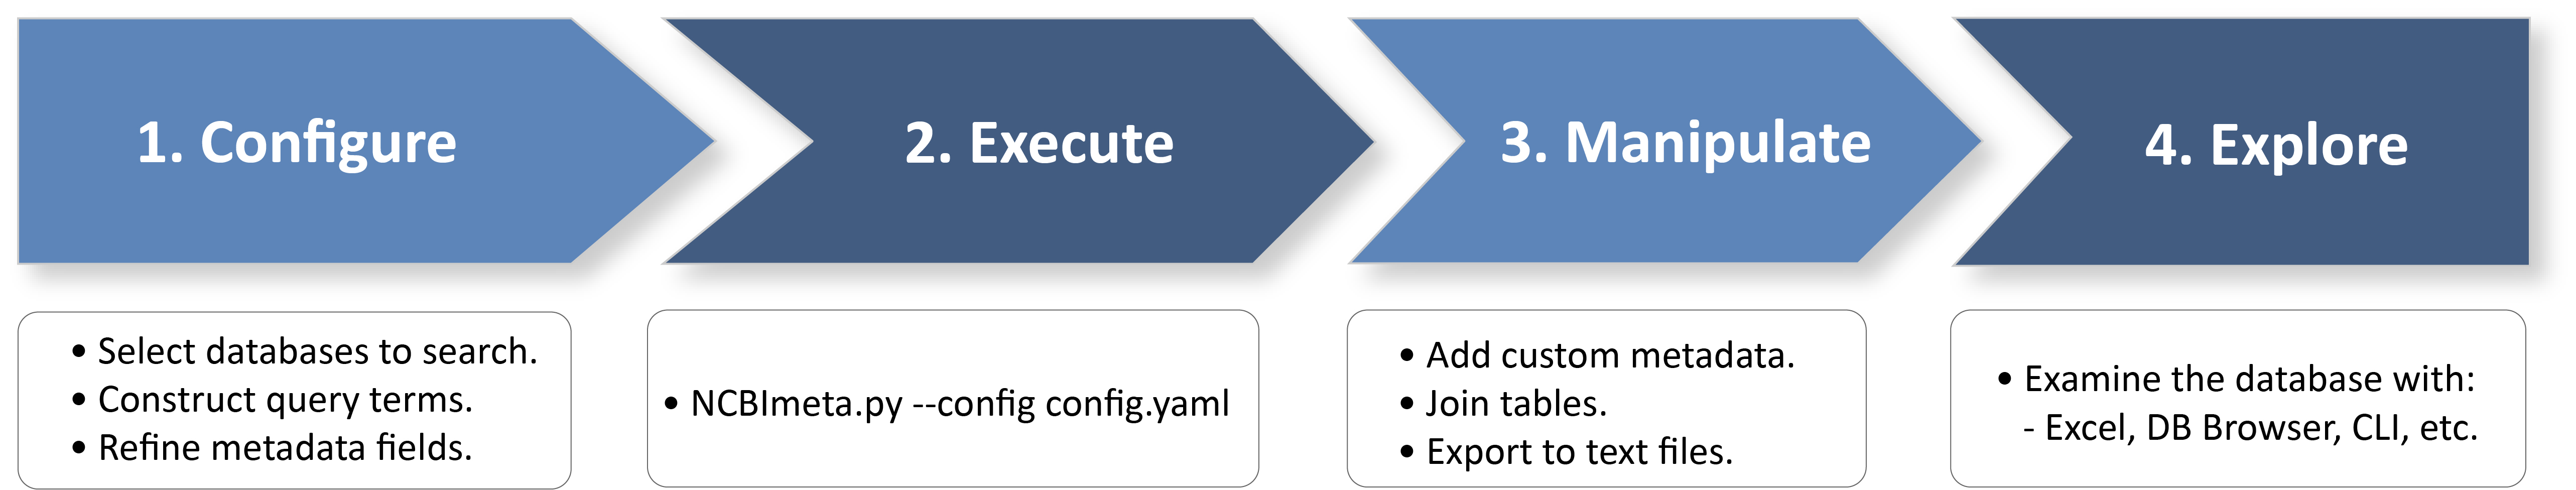
\includegraphics{https://rawcdn.githack.com/ktmeaton/NCBImeta/ae039b34/paper/figures/NCBImeta_Workflow.png}
\caption{Figure 1: NCBImeta user workflow.}\label{fig:NCBImeta_Workflow}
}
\end{figure}

\texttt{NCBImeta}'s implementation offers a novel approach to metadata
management and presentation that improves upon the prevously described
limitations of existing software in a number of ways. First,
\texttt{NCBImeta} is run on the command-line, and the final database can
be exported to a text file, thus no knowledge of an external programming
language is required to generate or explore the output. Second, a
general parsing framework for tables and metadata fields was developed
which can be extended to work with diverse database types contained
within NCBI's infrastructure. Finally, a query system was implemented
for record retrieval that allows users to access records in real-time,
as opposed to working with intermittent or out-dated database snapshots.

\hypertarget{sec:use-case}{%
\subsection{Use Case}\label{sec:use-case}}

The following section demonstrates how \texttt{NCBImeta} can be used to
obtain current and comprehensive metadata for a pathogenic bacteria,
\emph{Pseudomonas aeruginosa}, from various sequencing projects across
the globe. \emph{P. aeruginosa} is an opportunistic pathogen associated
with the disease cystic fibrosis (CF) and is highly adaptable to diverse
ecological niches (Stewart et al., 2014). As such, it is a target of
great interest for comparative genomics and there are currently over
15,000 genomic sequence records available which are spread across two or
more databases. In cases such as this, it is critical to leverage the
tremendous power of these existing datasets while being conscious of the
labor typically required to retrieve and contextualize this information.
\texttt{NCBImeta} renders the problem of acquiring and sifting through
this metadata trivial and facilitates the integration of information
from multiple sources.

To identify publicly available \emph{P. aeruginosa} genomes,
\texttt{NCBImeta} is configured to search through the tables
\emph{Assembly} (assembled genomes) and \emph{SRA} (raw data). For
additional context, \texttt{NCBImeta} is used to retrieve metadata from
the \emph{Nucleotide} table for descriptive statistics of the genomic
content, from the \emph{BioProject} table to examine the research
methodology of the initiative, from \emph{Pubmed} to identify existing
publications, and finally from the \emph{Biosample} table to explore
characteristics of the biological material. A small subset of the 100+
retrieved columns is shown in Figure~2, to provide a visual example of
the output format and the metadata that is retrieved.

\begin{figure}
\hypertarget{fig:NCBImeta_aeruginos_db_subset}{%
\centering
\includegraphics{https://rawcdn.githack.com/ktmeaton/NCBImeta/ae039b348f433/paper/figures/NCBImeta_aeruginosa_geogene.png}
\caption{Figure 2: A subset of the 100+ metadata columns retrieved for
\emph{P. aeruginosa} sequencing projects. Viewed with DB Browser for
SQLite
(https://sqlitebrowser.org/).}\label{fig:NCBImeta_aeruginos_db_subset}
}
\end{figure}

Subsequently, the output of NCBImeta can be used for exploratory data
visualization and analysis. The text file export function of NCBImeta
ensures downstream compatibility with both user-friendly online tools
(ex. Google Sheets Charts) as well as more advanced visualization
packages (Wickham, 2016). In Figure~3, the geospatial distribution of
\emph{P. aeruginosa} isolates are plotted alongside key aspects of
genomic composition (ex. number of genes).

\begin{figure}
\hypertarget{fig:NCBImeta_aeruginosa_geogene}{%
\centering
\includegraphics{https://rawcdn.githack.com/ktmeaton/NCBImeta/ae039b348/paper/figures/NCBImeta_aeruginosa_geogene.png}
\caption{Figure 3: Metadata visualization of \emph{P. aeruginosa}
sequencing projects. A) The geographic distribution of samples in this
region highlights a large number originating in Japan. Visualized with
Palladio (https://hdlab.stanford.edu/palladio/). B) The number of genes
per organism reveals a multi-modal distribution within the
species.}\label{fig:NCBImeta_aeruginosa_geogene}
}
\end{figure}

Finally, NCBImeta can be used to streamline the process of primary data
acquisition following careful filtration. FTP links are provided as
metadata fields for databases attached to an FTP server (ex. Assembly,
SRA) which can be used to download biological data for downstream
analysis.

\hypertarget{sec:future-work}{%
\subsection{Future Work}\label{sec:future-work}}

The development of \texttt{NCBImeta} has primarily focused on a target
audience of researchers whose analytical focus is prokaryotic genomics
and the samples of interest are the organisms themselves. Chief among
those include individuals pursuing questions concerning epidemiology,
phylogeography, and comparative genomics. Future releases of
\texttt{NCBImeta} will seek to broaden database representation to
include gene-centric and transcriptomics research (ex. NCBI's Gene and
GEO databases).

\hypertarget{sec:availability}{%
\subsection{Availability}\label{sec:availability}}

NCBImeta is a command-line application written in Python 3 that is
supported on Linux and macOS systems. It is distributed for use under
the OSD-compliant MIT license (https://opensource.org/licenses/MIT).
Source code, documentation, and example files are available on the
GitHub repository (https://github.com/ktmeaton/NCBImeta).

\hypertarget{sec:acknowledgements}{%
\subsection{Acknowledgements}\label{sec:acknowledgements}}

I would like to thank Dr.~Hendrik Poinar and Dr.~Brian Golding for their
guidance and support on this project, as well as for insightful
conversations regarding biological metadata, the architecture of NCBI,
and software deployment. Thank you to Dr.~Andrea Zeffiro, Dr.~John Fink,
Dr.~Matthew Davis, and Dr.~Amanda Montague for valuable discussions
regarding APIs, digital project management, and software publishing.
Thank you to all past and present members of the McMaster Ancient DNA
Centre and the Golding Lab. This work was supported by the MacDATA
Institute (McMaster University, Canada) and the Social Sciences and
Humanities Research Council of Canada (\#20008499).

\hypertarget{sec:references}{%
\subsection*{References}\label{sec:references}}
\addcontentsline{toc}{subsection}{References}

Bernstein, M. N., Doan, A., \& Dewey, C. N. (2017). MetaSRA: Normalized
human sample-specific metadata for the Sequence Read Archive.
\emph{Bioinformatics}, \emph{33}(18), 2914--2923.
\url{https://doi.org/10.1093/bioinformatics/btx334}

Chang, W. E., Peterson, M. W., Garay, C. D., \& Korves, T. (2016).
Pathogen metadata platform: Software for accessing and analyzing
pathogen strain information. \emph{BMC Bioinformatics}, \emph{17}(1).
\url{https://doi.org/10.1186/s12859-016-1231-2}

Choudhary, S. (2019). Pysradb: A Python package to query next-generation
sequencing metadata and data from NCBI Sequence Read Archive.
\emph{F1000Research}, \emph{8}, 532.
\url{https://doi.org/10.12688/f1000research.18676.1}

Cock, P. J. A., Antao, T., Chang, J. T., Chapman, B. A., Cox, C. J.,
Dalke, A., Friedberg, I., Hamelryck, T., Kauff, F., Wilczynski, B., \&
de Hoon, M. J. L. (2009). Biopython: Freely available Python tools for
computational molecular biology and bioinformatics.
\emph{Bioinformatics}, \emph{25}(11), 1422--1423.
\url{https://doi.org/10.1093/bioinformatics/btp163}

Connor, T. R., Barker, C. R., Baker, K. S., Weill, F.-X., Talukder, K.
A., Smith, A. M., Baker, S., Gouali, M., Pham Thanh, D., Jahan Azmi, I.,
Dias da Silveira, W., Semmler, T., Wieler, L. H., Jenkins, C., Cravioto,
A., Faruque, S. M., Parkhill, J., Wook Kim, D., Keddy, K. H., \&
Thomson, N. R. (2015). Species-wide whole genome sequencing reveals
historical global spread and recent local persistence in \emph{Shigella}
\emph{Flexneri}. \emph{eLife}, \emph{4}.
\url{https://doi.org/10.7554/eLife.07335}

\emph{Entrez Help}. (2016). National Center for Biotechnology
Information.

Eppinger, M., Pearson, T., Koenig, S. S. K., Pearson, O., Hicks, N.,
Agrawal, S., Sanjar, F., Galens, K., Daugherty, S., Crabtree, J.,
Hendriksen, R. S., Price, L. B., Upadhyay, B. P., Shakya, G., Fraser, C.
M., Ravel, J., \& Keim, P. S. (2014). Genomic epidemiology of the
Haitian cholera outbreak: A single introduction followed by rapid,
extensive, and continued spread characterized the onset of the epidemic.
\emph{mBio}, \emph{5}(6). \url{https://doi.org/10.1128/mBio.01721-14}

Kans, J. (2019). Entrez Direct: E-utilities on the UNIX Command Line. In
\emph{Entrez Programming Utilities Help}. National Center for
Biotechnology Information.

Mackenzie, A., McNally, R., Mills, R., \& Sharples, S. (2016).
Post-archival genomics and the bulk logistics of DNA sequences.
\emph{BioSocieties}, \emph{11}(1), 82--105.
\url{https://doi.org/10.1057/biosoc.2015.22}

Nakazato, T., Ohta, T., \& Bono, H. (2013). Experimental design-based
functional mining and characterization of high-throughput sequencing
data in the Sequence Read Archive. \emph{PLoS ONE}, \emph{8}(10),
e77910. \url{https://doi.org/10.1371/journal.pone.0077910}

Stewart, L., Ford, A., Sangal, V., Jeukens, J., Boyle, B.,
Kukavica-Ibrulj, I., Caim, S., Crossman, L., Hoskisson, P. A., Levesque,
R., \& Tucker, N. P. (2014). Draft genomes of 12 host-adapted and
environmental isolates of \emph{Pseudomonas} \emph{Aeruginosa} and their
positions in the core genome phylogeny. \emph{Pathogens and Disease},
\emph{71}(1), 20--25. \url{https://doi.org/10.1111/2049-632X.12107}

Wickham, H. (2016). \emph{Ggplot2: Elegant Graphics for Data Analysis}.
Springer-Verlag.

Zankari, E., Hasman, H., Cosentino, S., Vestergaard, M., Rasmussen, S.,
Lund, O., Aarestrup, F. M., \& Larsen, M. V. (2012). Identification of
acquired antimicrobial resistance genes. \emph{Journal of Antimicrobial
Chemotherapy}, \emph{67}(11), 2640--2644.
\url{https://doi.org/10.1093/jac/dks261}

Zhu, Y., Stephens, R. M., Meltzer, P. S., \& Davis, S. R. (2013). SRAdb:
Query and use public next-generation sequencing data from within R.
\emph{BMC Bioinformatics}, \emph{14}(1), 19.
\url{https://doi.org/10.1186/1471-2105-14-19}

\hypertarget{plague-denmark}{%
\section{Plague Denmark}\label{plague-denmark}}

% %%%%%%%%%%%%%%%%%%%%%%%%%%%%%%%%%%%%%%%%%%%%%%%%%%%%%%%%%
% Appendix
\begin{appendix}
\end{appendix}


\label{NumDocumentPages}

\end{document}
